\section{Rychlost vykreslování}
Jednou z otázek, na kterou se snaží najít odpověď tento VÚ je to, zda by bylo možné odstranit z programu knihovny Cg, OpenGL. Bylo tedy potřeba zjistit, jaký dopad by mělo odstranění knihoven OpenGL, Cg na funkčnost programu. Jedná se o knihovny usnadňující vykreslování obrazových dat. Zároveň se ale jedná o knihovny urychlující vykreslování dat. Při odstranění knihoven by se tak mohlo stát, že program nebude schopen dostatečně rychle vizualizovat data a nebude tak možné v reálném čase vykreslovat to, co uživatel dělá.

Pro zjištění toho, jaký dopad bude mít absence knihoven na výkon, bylo potřeba nějakým způsobem změřit rychlost renderování s využitím grafických knihoven a bez nich. K tomuto účelu byly zkonstruovány tři testovací programy, každý z nich obohacen o podporu nějaké specifické grafické knihovny. První program využíval jen grafickou podporu v knihovně Qt, druhý využíval podpory Qt a OpenGL, třetí pak všech tří knihoven: Qt, OpenGL, Cg toolkit. Jako cíl programů bylo stanoveno změnit světlost snímku a vykreslit jej na obrazovku. Aby bylo možné naměřit relevantní data, necháme operaci běžet v cyklech několikrát za sebou.

Pro zjištění toho, jaký dopad na funkčnost programu bude mít absence knihovny OpenGL, respektive Cg, byly nejprve zkonstruovány tři testovací programy. Všechny tři programy měli za cíl co nejvíckrát za sebou vykreslit stejný snímek, v každém kroku ale provedli se snímkem jednoduchou barevnou úpravu. Programy se lišili v tom, které z knihoven využívali. První se opíral jen o grafické funkce Qt knihovny, druhý využíval k vizualizaci Qt i OpenGL, třetí pak Qt, OpenGL i Cg toolkit. Smyslem bylo porovnat rychlost vykreslování všech tří variant. Jako testovací grafickou operaci jsme si vybrali jednoduché násobení všech barevných složek každého pixelu konstantou.

Výsledky testování vypovídaly o značném zpomalení při nepřítomnosti knihovny OpenGL v programu. Z toho se daly vyvozovat závěry, že knihovnu OpenGL nebude možné z programu odstranit (viz závěr této kapitoly - řádové zpomalení). Nicméně po konzultaci se školitelem, se podařilo objevit implementaci stejné úlohy pouze v knihovně OpenGL, která však byla téměř o řád rychlejší. Vzhledem k tomu, že pomalejší implementace je intuitivnější, zatímco rychlejší tak intuitivní neni, ale využívá hlubších poznatků problematiky datové reprezentace ukládání snímků, uvádíme obě implementace.

\begin{tabular}{| l | l | }
  \hline                       
  Varianta 1 & Qt\\
  \hline
  Varianta 2 & Qt, OpenGL\\
  \hline
  Varianta 3 & Qt, OpenGL, Cg toolkit \\
  \hline  
\end{tabular}

\subsection{Implementace v Qt}
Grafická část rozhraní knihovny Qt je dělaná čistě pro dvojrozměrnou grafiku a všechny výpočty jsou prováděny jen na procesoru. Chceme-li měnit světlost snímku, musíme procházet for-cyklem všechny body obrázku a provést operaci pro každý bod zvlášť. Pokud navíc zadáme světlost pixelu mimo požadovanou mez, program se zasekne. Narozdíl od toho knihovny OpenGL i Cg automaticky barevnou hodnotu pixelu oříznou na přípustnou mez.

Intuitivní, avšak pomalejší implementace v Qt knihovně vypadá následovně:

\begin{lstlisting}[label=DicomImageClass,caption={...}]
	start = time (NULL);
	QLabel label;
	QImage MemoryImage("D:/Workspace/Qt/Picture.png");
	QImage ShowImage("D:/Workspace/Qt/Picture.png");
	label.setPixmap(QPixmap::fromImage(ShowImage));
	label.show();
	qreal H, S, V;
	QColor Color;
	qreal contrast=0;
	for (int j=0; j<10; j++){
		cont = 0;
		for (int i=0; i<99; i++){
			cont=cont+0.01;
			ShowImage = MemoryImage;
			for ( int y = 0; y < h; y++ ){
				for ( int x = 0; x < w; x++ ){
					Rgb = MemoryImage.pixel(x,y);
					Rgb = qRgb(qRed(Rgb)*cont,qGreen(Rgb)*cont,qBlue(Rgb)*cont);
					ShowImage.setPixel(x,y,Rgb);
				}
			}
			label.setPixmap(QPixmap::fromImage(ShowImage));
			label.repaint();
		}
	}
	end = time (NULL);
\end{lstlisting}

V úryvku kódu vidíme zejména procházení celého obrázku ve dvou for-cyklech(řádky 13,14). V každém kroku si zjistíme barevné souřadnice pixelu, upravíme je a uložíme je. To má na starosti procesor a jedná se o největší handicap celého programu. Při této implementaci je úloha zpracována sériově na jednom jádře, jak je vidět z následujících grafů sledujících zátěž jednotlivých jader:

\hspace{1cm}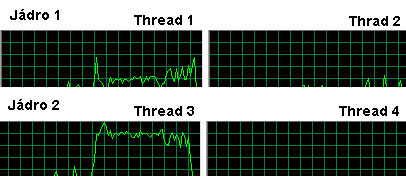
\includegraphics[width=0.8\textwidth]{Text/IMG/MultiThread.jpg}

Procesor je fyzicky dvoujádrový, ale operační systém jej vidí jako čyřjádrový. Celý výpočet probíhal viditelně v třetím threadu, v prvním pak běžely zřejmě jen pomocné operace, další 2 thready zůstaly nevyužité.

Chceme-li výpočet urychlit, můžeme tak udělat v několika krocích:

Nebudeme si ukládat barevné souřadnice původního obrázku do proměnné, tam je upravovat a ukládat zpět na půbodní místo. Ale necháme si předat ukazatel na místo v paměti, kde je obrázek uložen, a výsledek ukládat přímo tam.

Dále nebudeme volat funkci, která nám na základě souřadnic vrátí barevné složky obrázku, ale necháme si od Qt knihovny předat ukazatel na celý jeden řádek obrázku. Tím se vyhneme opakovanému volání funkce.

Dvojice for-cyklů procházející obrázek bude nahrazena tímto kódem:

\begin{lstlisting}[label=DicomImageClass,caption={...}]
for (int i=0; i<99; i++){
	cont=cont+0.01;
	ShowImage = MemoryImage;
	for ( int y = 0; y < h; y++ ){
		Rgb = (QRgb*)ShowImage.scanLine(y);
		for ( int x = 0; x < w; x++ ){
			Rgb[x] = qRgb(qRed(Rgb[x])*cont,qGreen(Rgb[x])*cont,qBlue(Rgb[x])*cont);
		}
	}
	label.setPixmap(QPixmap::fromImage(ShowImage));
	label.repaint();
}
\end{lstlisting}

Jak je vidět, v každém řádku obrázku ušetříme hned dvě volání funkce pro každý pixel. Zkusme si spočítat kolik funkčních volání jsme ušetřili:

V prvním případě voláme pro každý pixel funkce QImage::pixel() a QImage::setPixel(). Rozměr obrázku je 512*512 pixelů. To jest: 512*512*2 = cca 500 000 funkčních volání.

V druhém případě voláme pouze funkci QImage::scanLine pro každý řádek obrázku, tj. 512*2 = 1024 volání.

Jak je vidět, jedná se o zredukování počtu volání nějaké funkce o dva řády. Výsledek takového zjednodušení uvidíme v závěru kapitoly.


\subsection{Implementace v OpenGL}

OpenGL je knihovna přímo určená pro urychlení grafických výpočtů a jejich zjednodušenou obsluhu. Hlavní rozdíl oproti implementaci v Qt je ten, že výpočty neprobíhají na procesoru, ale na grafické kartě, což je, jak se později ukáže, zásadní rozdíl ve výkonnosti programu. Stejně tak data nejsou uložena v modulech paměti RAM na základní desce, ale jsou v paměti grafické karty.

Implementace vypadá následovně:

\begin{lstlisting}[label=DicomImageClass,caption={...}]
start = time (NULL);
for (int j=0; j<10; j++){
	float Brightness=0.0;
	for (int i=0; i<1000; i++){
		Brightness = Brightness+0.001;
		gl->Paint(Brightness);
		w.updateGL();
	}
}
end = time (NULL);

void GLPainter::PrepareTexture() {
	glBindTexture( GL_TEXTURE_2D, TextureIdentifier );
	gluBuild2DMipmaps( GL_TEXTURE_2D, 3, width, height, GL_RGB, GL_UNSIGNED_BYTE, TextureData );
	glEnable( GL_TEXTURE_2D );
}

void GLPainter::Paint(float Brightness){
	glBegin(GL_POLYGON);
		glColor3f (Brightness, Brightness, Brightness);
		glTexCoord3f(0.0,0.0,0.0);	glVertex3f( -1.0, -1.0, 0.0 );
		glTexCoord3f(0.0,1.0,0.0);	glVertex3f( -1.0,  1.0, 0.0 );
		glTexCoord3f(1.0,1.0,0.0);	glVertex3f(  1.0,  1.0, 0.0 );
		glTexCoord3f(1.0,0.0,0.0);	glVertex3f(  1.0, -1.0, 0.0 );
	glEnd();
}
\end{lstlisting}
Na první pohled lze vidět nesrovnatelné zjednodušení kódu, zatímco v prvním případě (Qt) jsme museli procházet celý obrázek po pixelech, zde můžeme využít funkce knihovny OpenGL pomocí které lze měnit světlost jejího výstupu.

V programu si nejprve snímek uložíme do paměti jakožto OpenGL texturu (řádky 12-16), posléze provádíme vykreslování této textury na načrtnutý obdélník (18-26).


\subsection{Iplementace v Cg}

Knihovna Cg slouží k programování výpočtů na čipu grafické karty. V jednoduchém jazyku podobném jazyku C popíšeme prováděné výpočty pro změnu světlosti. Výpočty jsou pak realizovány na speciálním hardwarovém čipu (pixel shader, vertex shader). Přínos pixel a vertex shaderů je v nové paletě efektů, jež je možno provádět, a dále ve výrazném urychlení těchto efektů.

Podívejme se na implementaci programu s využitím Cg, tentokráte výpočty nebyly prováděny jen v prostředí jazyka C++, ale i v jazyce Cg.

\begin{lstlisting}[label=DicomImageClass,caption={...}]
start = time (NULL);
for (int j=0; j<10; j++){
	float Brightness=0.0;
	for (int i=0; i<1000; i++){
		Brightness = Brightness+0.001;
		gl->Paint(Brightness);
		w.updateGL();
	}
}
end = time (NULL);

void GLPainter::PrepareTexture() {
	glBindTexture( GL_TEXTURE_2D, TextureIdentifier );
	gluBuild2DMipmaps( GL_TEXTURE_2D, 3, width, height, GL_RGB, GL_UNSIGNED_BYTE, TextureData );
	glEnable( GL_TEXTURE_2D );
}

void GLPainter::changeBrightness( float Brightness ){
	cgGLBindProgram(Program);
	cgGLEnableProfile(Profile);
	cgSetParameter1f(hBright, Brightness);
	cgUpdateProgramParameters (Program);
	cgGLDisableProfile(Profile);

	Paint();
}

void GLPainter::Paint(){
	glClear(GL_COLOR_BUFFER_BIT);

	cgGLBindProgram(Program);
	cgGLEnableProfile(Profile);
	cgGLEnableTextureParameter(hDecal);

	glBegin(GL_POLYGON);
		glTexCoord3f(0.0,0.0,0.0);	glVertex3f(-1.0,-1.0,0.0);
		glTexCoord3f(0.0,1.0,0.0);	glVertex3f(-1.0,1.0,0.0);
		glTexCoord3f(1.0,1.0,0.0);	glVertex3f(1.0,1.0,0.0);
		glTexCoord3f(1.0,0.0,0.0);	glVertex3f(1.0,-1.0,0.0);
	glEnd();

	cgGLDisableProfile(Profile);
	cgGLDisableTextureParameter(hDecal);
}
\end{lstlisting}

\begin{lstlisting}[label=DicomImageClass,caption={...}]
struct C3E3f_Output {
  float4 color : COLOR;
};

C3E3f_Output main(float2 texCoord : TEXCOORD0, uniform sampler2D decal : TEX0, uniform float brightness)
{
  C3E3f_Output OUT;
  OUT.color = tex2D(decal,texCoord)*brightness;

  return OUT;
}
\end{lstlisting}

První část programu je shodná s předchozí verzí (opět je volána knihovna OpenGL). Rozdíl však začíná od řádku 18. Ve funkci changeBrightness() musíme volat funkce knihovny Cg toolkit pomocí kterých předáme pixel shaderu parametr určující změnu světlosti. Před samotným vykreslováním pomocí OpenGL (řádky 35-40) musíme nechat program zkompilovat na čipu grafické karty a nastavit, aby ovlivňoval výstup OpenGL.

Za povšimnutí stojí fakt, že výpočet změny světlosti se přesunul z kódu C++ do Cg. Změna světlosti je popsána v samostatném programu jež se kompiluje na grafické kartě.


\subsection{Porovnání výpočtů}

Popsané programy byly testovány na počítačové sestavě:

Intel Core i3, ATI Radeon 5470. Takt procesoru je 2,26 GHz

Jedná se o dvoujádrový procesor, pro výpočet však bylo použito pouze jedno jádro. Takt GPU na grafické kartě je 750MHz.

V každé konfiguraci jsme požadovali jiný počet cyklů programu, jenom z důvodu časové úspory při ladění.

\begin{tabular}{| p{5cm} | l | l | l | }
  \hline                       
  Typ konfigurace & Počet cyklů & Čas & Snímků za vteřinu \\
  \hline
  \hline
  Qt (bez přímého přístupu do paměti)& 100 & 4 sekundy & 25 fps\\
  \hline
  Qt (s přímým přístupem do paměti)& 1000 & 11 sekund & 90 fps\\
  \hline
  Qt, OpenGL & 10 000 & 16 sekund & cca 600  fps \\
  \hline
  Qt, OpenGL, Cg & 10 000 & 14 sekund & cca 700 fps \\
  \hline  
\end{tabular}

Jak je vidět z namšřených údajů, s použitím knihovny OpenGL se dá dosáhnout úctihodného výkonu při vykreslování snímků v programu. Nicméně vezmeme-li v úvahu fakt, že standardní rychlost snímání ovládacích zařízení přes USB v operačním systému je 125Hz a dále obnovovací frekvence u monitoru nebývá zpravidla vyšší než 100Hz, musíme uznat, že výkon dosažený pomocí OpenGL je nadbytečný. To by určitě nevadilo a velká rezerva ve výkonu by mohla být zárukou plynulého chodu programu i za ztížených podmínek (uživatel využívá procesor i jiným způsobem za běhu programu), ale bohužel přítomnost knihovny OpenGL v programu má za důsledek značné problémy s provozem programu na méně výkonných, či starších grafických kartách. Byly zjištěny problémy s provozem programu na integrovaných grafických kartách Intel, které však jsou velice často instalovány do moderních notebooků.

Výkon programu, při pomalejší implementaci v Qt knihovně, kdy jsme nevyužívali manuálního přístupu do paměti, ale k tomuto jsme používali implementované funkce v Qt knohovně, je spíše nedostačující. Dosažený výkon v testovacím programu: 25 snímků za vteřinu sice sám o sobě dostačující je, ale musíme vzít v úvahu ten fakt, že se jednalo o velice primitivní testovací program, který nedělal nic jiného než přepočet barevných složek obrázku a jeho zobrazení. DicomPresenter vedle toho musí vykreslovat ovládací prvky programu, což znamená několik funkčních volání navíc.

Oproti tomu výkon dosažený pomocí pokročilé implementace, kdy přistupujeme ručně do paměti počítače a obrazová data měníme tam, by měl být dostačující pro běh reálného programu. I při výrazném zpomalení aplikace kvůli přepočítávání zobrazovaných ovládacích prvků, bychom se měli bezpečně udržet nad hranicí 30FPS.

Závěrem této kapitoly je nutno podotknout, že Knihovny OpenGL, Cg z programu odstranit lze a v nejbližší době bude takto učiněno. Program by se tak měl stát výrazně bezproblémovější, co se týče provozu v praxi. Měl by být kompatibilní s převážnou většinou počítačových sestav - to je však nutná podmínka pro to, aby program mohl být v praxi použitelný.





